\documentclass{standalone}
\usepackage{tikz}
\usetikzlibrary{matrix,chains,positioning,decorations.pathreplacing,arrows}
\usetikzlibrary{positioning, calc, chains}
\begin{document}


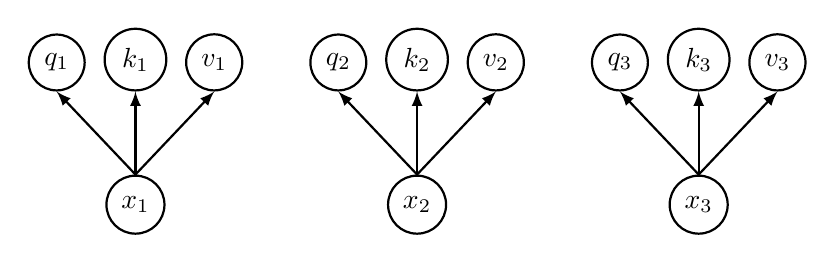
\begin{tikzpicture}[item/.style={circle,draw,thick,align=center},
itemc/.style={item,on chain,join}]
\begin{scope}[start chain, node distance=8em,  every node/.style={circle,draw, thick}]
\node [on chain] (x1) {$x_1$};
\node [on chain] (x2) {$x_2$};
\node [on chain] (x3) {$x_3$};
\end{scope}

\foreach \T in {1,2,3} 
{\draw[thick,-latex] (x\T.north) -- ++ (0,3em)
	node[above,item] (k\T) {$k_\T$};
 \draw[thick,-latex] (x\T.north) -- ++ (1,3em)
	node[above,item] (v\T) {$v_\T$};
\draw[thick,-latex] (x\T.north) -- ++ (-1,3em)
node[above,item] (q\T) {$q_\T$};
}
\end{tikzpicture}
\end{document}